\problemname{Kvicksand}
\noindent

Sandra har flyttat till Sandsvall för att studera. Efter att ha tillbringat några dagar i den
nya staden har Sandra märkt att det är kvicksand på flera platser. 
Om man åker till någon av dessa platser så fastnar man i sanden och kommer inte därifrån.
Sandra vill ha reda på exakt var kvicksanden finns så att hon kan undvika dessa platser.
Som tur är har Sandsvall, till skillnad från Göteborg, en välfungerande reseplaneringsapp.
Med hjälp av reseplaneraren har Sandra tagit reda på hur lång tid det tar att åka från 
hennes bostad till var och en av de andra platserna i staden.

Sandsvall kan representeras av en oriktad graf med $N$ noder och $M$ kanter. Sandras bostad
är på nod nummer $1$. Det tar en minut att åka mellan två noder som är sammankopplade med en kant.
En okänd mängd noder har kvicksand, och det går inte att åka från dessa noder även om de har kanter
till andra noder.

Du får givet talen $d_1, d_2, \dots, d_N$, där $d_i$ är hur många minuter det tar att åka från 
nod $1$ till nod $i$. Om det inte går att ta sig till nod $i$ överhuvudtaget så är $d_i = -1$.
Din uppgift är att med hjälp av denna information hitta vilka noder som har kvicksand.

\section*{Input}

Den första raden innehåller två heltal $N$ och $M$ ($2 \leq N \leq 3 \cdot 10^5$, $N-1 \leq M \leq 3 \cdot 10^5$).

Den andra raden innehåller de $N$ heltalen $d_1, d_2, \dots, d_N$ ($-1 \leq d_i \leq N$). Det första talet
$d_1$ kommer alltid att vara noll.

De följande $M$ raderna innehåller två heltal $u_i, v_i$ ($1 \leq u_i, v_i \leq N$, $u_i \neq v_i$), vilket innebär
att det går en kant mellan $u_i$ och $v_i$. Det kommer finnas högst en kant mellan varje par av noder.
Grafen kommer alltid vara sammanhängande, vilket betyder att det går att gå till alla noder 
med en sekvens av kanter (däremot kan kvicksanden göra att det är omöjligt att nå vissa noder).

\section*{Output}

Om det inte finns något möjligt sätt för kvicksanden att vara fördelad som stämmer överens med 
informationen, skriv ut $-1$.

Annars, skriv först ut ett heltal $K$ ($0 \leq K \leq N$), antalet noder som har kvicksand.
Skriv därefter ut $K$ olika heltal $a_1, a_2, \dots, a_K$, indexen på de noder som har kvicksand.
Om det finns flera möjligheter så kan du skriva ut vilken som helst av dem.

\section*{Poängsättning}
Din lösning kommer att testas på en mängd testfallsgrupper.
För att få poäng för en grupp så måste du klara alla testfall i gruppen.

\noindent
\begin{tabular}{| l | l | p{12cm} |}
  \hline
  \textbf{Grupp} & \textbf{Poäng} & \textbf{Gränser} \\ \hline
  $1$    & $17$        & Svaret är aldrig $-1$ och grafen är en linjegraf, dvs $M = N-1$ och kanterna är $(1, 2), (2, 3), \dots, (N-1, N)$\\ \hline
  $2$    & $29$        & Svaret är aldrig $-1$ och grafen är ett träd, dvs $M = N-1$. \\ \hline
  $3$    & $34$        & Svaret är aldrig $-1$. \\ \hline
  $4$    & $20$        & Inga ytterligare begränsningar. \\ \hline
\end{tabular}

\section*{Förklaring av exempelfall}

\begin{figure}[h!]
  \centering
  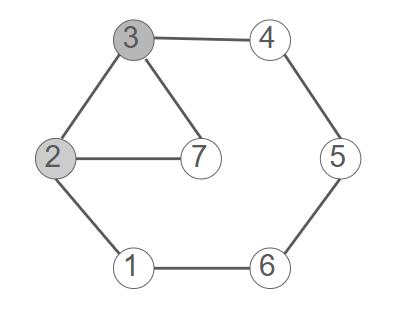
\includegraphics[width=0.3\textwidth]{kvicksand.PNG}
  \caption{Grafen i exempel 1.}
\end{figure}

I exempel 1 är det möjligt att $2$ och $3$ har kvicksand, som bilden visar. Då blir exempelvis 
nod $7$ omöjlig att nå. Nod $7$ skulle också kunna ha kvicksand, så ett annat möjligt svar är $2,3,7$.
